% =====================================================================================
%  Sec. 2 -- One sampling primitive, four channels: what is reconstructed from shots.
%
%  REPLACES release/paper/method.tex IN FULL.  It keeps that file's three labels
%  (sec:method, eq:lehmann, eq:green), which are referenced from results.tex,
%  hardware.tex, sec_3_1.tex, sec_4.tex and sec_8.tex, and keeps its whole citation
%  lineage.  It drops the closing sentence of method.tex (lines 82-88) that invoked the
%  retracted Theorem 1(iii), and installs in its place the drop-in agreed in sec_3_1.tex.
%
%  LABELS DEFINED HERE:  sec:method (kept)  eq:lehmann (kept)  eq:green (kept)
%                        sec:method:krylov  sec:method:rr  sec:method:provenance
%                        sec:method:budgets  eq:ritz  tab:provenance
%
%  EXTERNAL LABELS USED (must exist in the v3 tree):
%    thm:leakage  eq:twobudget  sec:leakage  sec:retraction        [Sec. 3]
%    sec:moments  thm:moments   prop:shots                         [Sec. 4, sec_4.tex]
%    sec:frontier                                                  [Sec. 5]
%    sec:nogo                                                      [Sec. 6, sec_6.tex]
%    sec:prices   tab:finiteshot                                   [Sec. 7, sec_7.tex]
%    sec:honest                                                    [discussion.tex, EXISTS]
%    fig:circ fig:method fig:hero fig:heron fig:lattice fig:akwsampled
%    fig:sqw fig:spin fig:scaling  tab:molecules                   [all EXIST in the tree]
%
%  FLOAT MOVED, CAPTION UNCHANGED: the fig:circ float is reproduced at the end of this
%  file exactly as it stands at hardware.tex:19-28, because Sec. 2 is now where it is
%  first referenced and it must land on the same page spread.
%  *** DELETE the float from hardware.tex when this file is installed, or \label{fig:circ}
%      is defined twice. ***
%
%  %TODO(results.tex:85): the clause "not the exact target of Fig.~\ref{fig:lattice}, but
%  the \emph{sampled} output" in the caption of fig:akwsampled is superseded by the
%  rebuilt caption (p2_figs/fig5_caption.tex) and by Table~\ref{tab:provenance} here.  It
%  must not survive anywhere in the v3 tree.
%
%  %TODO(abstract): the published abstract of v1-v2 reads, verbatim (checked against the
%  deposited submission tarball), "we reconstruct, from sampled subspaces, the
%  single-particle spectral function A(omega) and its momentum-resolved form A(k,omega);
%  the same primitive TARGETS the neutral-sector dynamical structure factors S(q,omega)
%  and S^zz(q,omega)".  Only the A(k,omega) half of the first clause is wrong, and this
%  section is its repair; the "targets" clause is already correct and must not be turned
%  into a confession that was never owed.  See the report.
%
%  DEPOSIT, checked 2026-09-18: DISCHARGED.  release/data/sampled_honest.json and
%  release/data/honest_sampling.json are both present, with sampled_honest.py and
%  honest_sampling_scaling.py in release/src/.  The shot budgets this table quotes are
%  regenerable from the deposit.
% =====================================================================================

\section{One sampling primitive, four channels: what is reconstructed from shots, and what is not}
\label{sec:method}

This section states the measurement primitive, fixes the one definition the rest of the paper turns on,
and then says --- channel by channel, figure by figure --- which objects here were reconstructed from a
finite number of measurements and which are full-sector references computed classically. Versions~1
and~2 of this preprint (arXiv:2608.16436) drew that line nowhere in the text, and one clause of the
abstract they carry draws it in the wrong place. It is drawn here, before any result is quoted.

\subsection{Construction}
For a Hamiltonian $\hat H$ with $N$-electron ground state $\lvert 0\rangle$ of energy $E_0$, the
single-particle spectral function has an electron-addition and an electron-removal branch,
\begin{equation}
\begin{aligned}
A_{p}(\omega)=&\sum_{n}\bigl|\langle n^{N+1}\lvert \hat c^\dagger_p\rvert 0\rangle\bigr|^{2}\,
\delta\!\bigl(\omega-(E^{N+1}_n-E_0)\bigr)\\
+&\sum_{m}\bigl|\langle m^{N-1}\lvert \hat c_p\rvert 0\rangle\bigr|^{2}\,
\delta\!\bigl(\omega-(E_0-E^{N-1}_m)\bigr),
\end{aligned}
\label{eq:lehmann}
\end{equation}
energies measured from $E_0$; the chemical potential $\mu=\tfrac12(E^{N+1}_0-E^{N-1}_0)$ places the
Fermi level mid-gap for the particle--hole-symmetric Hubbard model at half filling. The subspace is
built in three steps. \emph{(1)}~Prepare the response seeds
$\lvert\phi^{\pm}\rangle=\hat c^{\dagger}_p\lvert 0\rangle,\ \hat c_p\lvert 0\rangle$ in the
$(N{\pm}1)$ sectors. \emph{(2)}~Time-evolve each, $\lvert\phi^{\pm}(t_k)\rangle=e^{-i\hat H
t_k}\lvert\phi^{\pm}\rangle$, and measure computational-basis bitstrings at each of the $K{+}1$
snapshots; the union of the \emph{distinct} bitstrings returned is the determinant subspace
$\mathcal S^{\pm}$. \emph{(3)}~Form $\hat H_{\mathcal S^{\pm}}=P_{\mathcal S^{\pm}}\hat H P_{\mathcal
S^{\pm}}$, diagonalize it as $\sum_m \tilde E^{\pm}_m\lvert\tilde m^{\pm}\rangle\langle\tilde
m^{\pm}\rvert$, and evaluate the Lehmann sum inside $\mathcal S^{\pm}$. The retarded Green's function is
then assembled entirely on the classical processor,
\begin{widetext}
\begin{equation}
G_{pq}(\omega)=\sum_{m}\frac{\langle 0\lvert \hat c_p\rvert\tilde m^{+}\rangle\langle\tilde m^{+}\lvert \hat
c^\dagger_q\rvert 0\rangle}{\omega-(\tilde E^{+}_m-E_0)+i\eta}
+\sum_{m}\frac{\langle 0\lvert \hat c^{\dagger}_q\rvert\tilde m^{-}\rangle\langle\tilde m^{-}\lvert \hat
c_p\rvert 0\rangle}{\omega-(E_0-\tilde E^{-}_m)+i\eta},
\label{eq:green}
\end{equation}
\end{widetext}
whose imaginary part is the Lorentzian-broadened $A_{pq}(\omega)$ at resolution $\eta$. The seed selects
the channel: charged seeds $\hat c^\dagger_q\lvert 0\rangle$ in the $(N{\pm}1)$ sectors give $A(\omega)$
and, by Fourier transform of $G_{pq}$, $A(k,\omega)$; number-conserving density and spin seeds
$\hat n_q\lvert 0\rangle,\ \hat S^z_q\lvert 0\rangle$ in the neutral $N$ sector give $S(q,\omega)$ and
$S^{zz}(q,\omega)$. The processor measures \emph{only} bitstrings. Figure~\ref{fig:circ} schematizes the
primitive --- what one circuit and one readout can address; Table~\ref{tab:provenance} states separately
what was actually run for each channel here.

\subsection{Relation to quantum subspace and Krylov methods}\label{sec:method:krylov}
In exact arithmetic the span of the time-evolved seeds is the order-$K$ polynomial Krylov
space~\cite{shen2023,kirby2023}, and diagonalizing $\hat H$ inside a subspace containing it is the route
of quantum subspace expansion~\cite{mcclean2017qse}, filter diagonalization~\cite{parrish2019} and
real-time quantum Krylov algorithms~\cite{cortesgray2022}, whose error theory is now
characterized~\cite{epperly2022}. What distinguishes the present method is that these states are used
not to \emph{estimate matrix elements}~\cite{bauer2016,endo2020,rungger2020,greenediniz2024,bespalova2025,onqse2024}
--- the step requiring Hadamard tests or quantum equation-of-motion measurements on the device --- but
as a \emph{sampling distribution} selecting a determinant
subspace~\cite{robledomoreno2025,kanno2023,skqd2025,teqsci2024,extsqd2025,adaptqsci,shirakawa2025},
extended since to embedded fragments and to auxiliary-field
post-processing~\cite{shajan2024,danilov2025}, and here lifted to the $(N{\pm}1)$ manifold and to a
frequency-resolved observable. That lineage stops at
energies and, at most, discrete levels: the closest published results are a QSCI quasiparticle band
structure returning discrete poles~\cite{ohgoe2025}, a molecular spectrum built from a neutral-sector
autocorrelation with classically projected long-time dynamics~\cite{santini2025}, and, from the
measured-overlap side rather than the sampled one, a dynamical structure factor of a Kitaev spin
liquid obtained by quantum subspace expansion~\cite{umeano2025}, or a hybrid quantum--classical
framework for many-fermion response and structure~\cite{du2026}. Closest on lattice models, Nogaki
\emph{et al.}~\cite{nogaki2025} apply symmetry-adapted SQD to ground-state \emph{energies}, and Wray
\emph{et al.}~\cite{wray2025} measure how SQD converges on a variable-length cuprate chain. The readout
is that of SQD, the circuits are those of sample-based Krylov
diagonalization~\cite{skqd2025,yoshioka2025,piccinelli2025}, and all dynamical information is assembled
classically through Eq.~\eqref{eq:green} by one continued-fraction
resolvent~\cite{haydock1972,golub2010}.

\subsection{What the subspace reconstruction is: Rayleigh--Ritz, not restriction}\label{sec:method:rr}
Step~\emph{(3)} is the definition the rest of this paper turns on, and versions~1--2 never stated it.
With $P_{\mathcal S}$ the orthogonal projector onto the span of the determinants in $\mathcal S$ and
$\phi$ the seed,
\begin{widetext}
\begin{equation}
A_{\mathcal S}(\omega)=\frac{\eta}{\pi}\,
\bigl\lVert\,\bigl(\omega+E_0+i\eta-H_{\mathcal S}\bigr)^{-1}P_{\mathcal S}\phi\,\bigr\rVert^{2},
\qquad H_{\mathcal S}=P_{\mathcal S}\hat HP_{\mathcal S},
\label{eq:ritz}
\end{equation}
\end{widetext}
the spectral function of the \emph{Rayleigh--Ritz operator} $P_{\mathcal S}\hat HP_{\mathcal S}$, whose
poles are the Ritz values $\tilde E_m$ of Eq.~\eqref{eq:green} --- not eigenvalues of $\hat H$ --- and
not the restriction of $A$ to a subset of its own eigenpairs. The reproduction repository computes
exactly this, at the small sizes by forming and diagonalizing the submatrix $\hat H[\mathcal S,\mathcal
S]$ and at the large ones by a matrix-free restricted matrix--vector product inside the same continued
fraction; the consequence is the mechanism of this paper: \emph{spectral weight the subspace retains is
not kept in place, it is moved in $\omega$}. Truncation does not delete Lehmann poles, it displaces every surviving one, so the
weight a subspace captures cannot by itself bound how far the reconstruction has moved --- which is why
the weight-only bound of versions~1--2 is retracted in Sec.~\ref{sec:retraction} and replaced, in
Theorem~\ref{thm:leakage}, by a bound carrying a second term indexed on the coupling
$P_{\mathcal S}\hat HQ_{\mathcal S}$ across the boundary of $\mathcal S$, with $Q_{\mathcal S}$ the
complementary projector --- exactly what Eq.~\eqref{eq:ritz} discards. Two corollaries are
used later. A determinant acts on $A_{\mathcal S}$ through $H_{\mathcal S}$ even carrying no seed
amplitude: at sector fraction $0.85$, $30.2\%$ of the selected determinants at $L=6$ and $36.9\%$ at
$L=8$ lie outside $\operatorname{supp}(\phi)$, add exactly nothing to the captured weight, and still
move the Ritz spectrum. And on the smallest subspace of \emph{unit} captured weight, $\mathcal
S^{\star}=\operatorname{supp}(\phi)$ of size exactly $(\tfrac12+\tfrac1L)\dim$, the relative $L_1$ error
of Eq.~\eqref{eq:ritz} is still $0.43$ at $L=6$ and $0.33$ at $L=8$ at $\eta=0.18\,t$
(Sec.~\ref{sec:retraction}).

\subsection{Provenance: what was reconstructed from shots, channel by channel}\label{sec:method:provenance}
Table~\ref{tab:provenance} gives, for every dynamical object in this paper, the subspace it was built on
and the measurements that built it. Three readings versions~1--2 permitted are corrected with it.

\paragraph{The neutral channels are references, not reconstructions.} $S(q,\omega)$ and
$S^{zz}(q,\omega)$ are computed here by a continued fraction over the \emph{entire} $N$-particle sector
of $853\,776$ determinants at $L=12$, at recursion depth $n_\ell=200$: no subspace is selected and no
shot is drawn, and the generating scripts say so in their own headers. The abstract of versions~1--2
states that the primitive \emph{targets} these two channels --- what Fig.~\ref{fig:circ} asserts, and
what the seed algebra supports --- and does not state that they were reconstructed from measurements;
they were not, nor were the $A(k,\omega)$ of Fig.~\ref{fig:lattice} or the $\mathrm{N_2}$ series of
Fig.~\ref{fig:hero}. A reference at finite recursion depth is not the exact spectral function either, so
its depth is quoted with it, and we quote no error that lies within a factor $20$ of the drift of its
own reference.

\paragraph{What the Born ranking is, and what it is not.} The two objects versions~1--2 described as
sampled without a budget --- Fig.~\ref{fig:akwsampled}(a,b) and the dashed curve of
Fig.~\ref{fig:scaling}(b) --- select $\mathcal S$ by sorting the accumulated Born weight
$\sum_{k}|\langle d\,|\,e^{-i\hat Ht_k}\phi\rangle|^{2}$ of the evolved state over the $K{+}1$ snapshots
and keeping the top fraction. That weight is the distribution the device draws from, not the
ground-state amplitudes and not the exact Lehmann residues, so the ranking is \emph{not} a clairvoyant
oracle: the repository contains one of those, in \texttt{amortized\_recovery.py}, and labels it as such
there. It is the infinite-shot limit $T\to\infty$ of the declared protocol, approached from above in
error by any finite budget --- at matched subspace size finite sampling is worse by $1.50\pm0.25$ at
$L=6$ and $1.96\pm0.12$ at $L=8$ (Table~\ref{tab:finiteshot}) --- and in that limit it selects nothing
the device could never return: no determinant it ranks carries exactly zero accumulated weight at
$L=6,8,10$ or $12$, and at $L=12$ no determinant of the whole sector does. What it is not is a
finite-shot experiment, and it must not be called one. The
replacement is measured and quoted with its budget: at $L=8$, $T=2.60\times10^{6}$ shots over $K{+}1=19$
snapshots reach sector fraction $0.835\pm0.0025$ at relative $L_1$ error $(4.81\pm0.27)\times10^{-3}$
over eight independent shot streams (Fig.~\ref{fig:akwsampled}(c)), and the measured ladder from
$2.4\times10^{4}$ to $1.9\times10^{7}$ shots for $L=6$ to $L=12$ is Fig.~\ref{fig:scaling}(c) and
Table~\ref{tab:shots}. \textbf{Declared gap:} no finite-shot run exists for the literal configuration of
Fig.~\ref{fig:akwsampled}(a,b) --- $\eta=0.18\,t$, $K=16$ snapshots, all sixteen momentum channels.
Panel~(c) is a measured surrogate at one seed and one resolution, not the same experiment, and nothing
here extrapolates from the one to the other.

\paragraph{What the a posteriori checks establish.} The branch sum rules $\int A_p^{\pm}\,d\omega$ are
identities of the ground state, not measurements of a reconstruction. Integrated on the grid the figures
use, at $L=6$ and $\eta=0.15\,t$, the exact and reconstructed addition branches carry $0.48659$ and
$0.48647$ --- agreement to $2.4\times10^{-4}$ relative, both falling $2.7\%$ short of the analytic
$1-\langle\hat n_p\rangle=0.5$ because Lorentzian tails of width $\eta$ leave the finite frequency
window. That is a genuine consistency check on a zeroth moment, and not an error bound. The certificate
is the two-sided bound of Theorem~\ref{thm:leakage}, and where it is non-vacuous is measured, not
asserted, in Sec.~\ref{sec:frontier} --- an essential property given that the classical hardness of a
specific instance is empirical rather than a theorem (Sec.~\ref{sec:honest}). What is guaranteed in
advance is narrower and survives intact: a subspace containing the order-$K$ Krylov space reproduces
that branch's exact spectral moments through order $2K{+}1$, and is realized with high probability by a
shot budget polynomial in the target support and independent of the Hilbert-space dimension
(Theorem~\ref{thm:moments} and Prop.~\ref{prop:shots}, Sec.~\ref{sec:moments}).

\subsection{The two budgets}\label{sec:method:budgets}
The two halves of this paper are the two terms of one inequality. With $Q_{\mathcal S}$ the projector
complementary to $P_{\mathcal S}$ and
$w_{\mathcal S}=\lVert P_{\mathcal S}\phi\rVert^{2}/\lVert\phi\rVert^{2}$, the upper branch of
Eq.~\eqref{eq:twobudget} reads
\begin{widetext}
\begin{equation*}
\lVert A-A_{\mathcal S}\rVert_{1}\ \le\ \bigl(\lVert\phi\rVert+\lVert P_{\mathcal S}\phi\rVert\bigr)
\Bigl(\ \underbrace{\lVert Q_{\mathcal S}\phi\rVert}_{\text{what shots buy}}
\ +\ \underbrace{\Lambda_{\mathcal S}(\eta)/\eta}_{\text{what they do not}}\ \Bigr).
\end{equation*}
\end{widetext}
The captured-weight term $\lVert Q_{\mathcal S}\phi\rVert=\lVert\phi\rVert\sqrt{1-w_{\mathcal S}}$ is
what shots buy:
it vanishes as the sampler exhausts the Born support of the probe, and Table~\ref{tab:provenance} prices
that exhaustion in measurements. The leakage term $\Lambda_{\mathcal S}(\eta)/\eta$ is what they do not
buy. On the subspace that \emph{is} that support --- $\mathcal S^{\star}=\operatorname{supp}(\phi)$, of
size exactly $(\tfrac12+\tfrac1L)\dim$, fixed by the probe and not by any ranking, so that
$w_{\mathcal S}=1$ exactly by construction, with no tie-breaking and no zero-amplitude padding --- the
weight term is identically zero and the relative error is still $0.43$ at $L=6$ and $0.33$ at $L=8$ at
$\eta=0.18\,t$, rising to $1.15$ and $0.90$ at $\eta=0.05\,t$. $\Lambda_{\mathcal S}(\eta)$ is defined
by the resolvent at resolution $\eta$ and exists only inside the spectral half of this work: the
obstruction theorem of Sec.~\ref{sec:nogo} takes it as its subject and would have no subject without
Sec.~\ref{sec:leakage}. Conversely, Sec.~\ref{sec:leakage} leaves open precisely the question
Sec.~\ref{sec:nogo} answers --- whether the a posteriori certificate can be replaced by an a priori
predictor computed from the state. Neither half can be removed without leaving the other incomplete in
a way we can name.

% -------------------------------------------------------------------------------------
%  THE PROVENANCE TABLE
% -------------------------------------------------------------------------------------
\begin{table*}[tp]\centering\small
\caption{\textbf{Provenance of every dynamical object in this paper: the subspace it was built on, and
the measurements that built it.} ``Full sector'' means no subspace selection of any kind --- the
continued fraction runs on the whole sector at the stated recursion depth $n_\ell$, so the row is a
reference against which reconstructions are scored, not a reconstruction. ``Observed bitstrings'' means
the subspace is the union of the distinct bitstrings actually returned by $T$ draws split evenly over
the $K{+}1$ snapshots, which is the protocol of Sec.~\ref{sec:method}; one \emph{stream} is one
independent pseudorandom realization of that draw. ``Born ranking'' means the subspace is the top
fraction of the sector under the accumulated Born weight of the evolved state, which is the
$T\to\infty$ limit of the same protocol and carries no shot budget. Sector dimensions are exact; budgets
are per channel and per stream.}
\label{tab:provenance}
\setlength{\tabcolsep}{4pt}
\setlength{\parskip}{0pt}
\renewcommand{\arraystretch}{1.15}
\begin{tabular}{@{}p{0.225\linewidth}p{0.115\linewidth}p{0.315\linewidth}p{0.225\linewidth}@{}}
\toprule
\raggedright \textbf{Channel and system} & \raggedright \textbf{Shown in} & \raggedright \textbf{Determinant subspace} & \raggedright \textbf{Shots $T$}\tabularnewline
\midrule
\raggedright $A(\omega)$; Hubbard $L{=}6$, $U/t{=}8$, $\eta{=}0.15\,t$; $\dim=300$
 & \raggedright Fig.~\ref{fig:method}
 & \raggedright observed bitstrings; $|\mathcal S|=245$ of $300$ in panel~(a), $242.5$ on average in panel~(b)
 & \raggedright $5.2\times10^{4}$ per stream ($4\times10^{3}$ at each of $13$ snapshots, $K{=}12$), $8$ streams\tabularnewline
\raggedright $A(\omega)$, orbital projected; $19$ molecules at dissociation; $\dim=2$--$300$
 & \raggedright Table~\ref{tab:molecules}
 & \raggedright observed bitstrings; the fraction $|\mathcal S|/D$ is the last column of that table
 & \raggedright $2.16\times10^{5}$ per molecule ($8\times10^{3}$ at each of $27$ snapshots, $K{=}26$), one stream\tabularnewline
\raggedright $A(\omega)$; $\mathrm{N_2}$ along dissociation, CAS$(6,6)$
 & \raggedright Fig.~\ref{fig:hero}(a)
 & \raggedright full CAS sector
 & \raggedright none\tabularnewline
\raggedright $A(\omega)$; hardware, \texttt{ibm\_fez}, $L{=}6$, $U/t{=}4$, $\eta{=}0.15\,t$; $\dim=300$
 & \raggedright Fig.~\ref{fig:heron}(a)
 & \raggedright recovered from device bitstrings; $|\mathcal S|=300$ of $300$, the entire sector, so the agreement
   with the exact curve is exact by coverage and is not a fidelity measurement
 & \raggedright $5\times10^{4}$, pooled over the $t{=}0$ reference and $K{=}7$ evolution circuits\tabularnewline
\midrule
\raggedright $A(k,\omega)$; $L{=}12$, $\eta{=}0.18\,t$; $\dim=731\,808$
 & \raggedright Fig.~\ref{fig:lattice}
 & \raggedright full sector, $n_\ell=150$ per momentum
 & \raggedright none\tabularnewline
\raggedright $A(k,\omega)$; $L{=}8$, $\eta{=}0.18\,t$; $\dim=3920$
 & \raggedright Fig.~\ref{fig:akwsampled}(a,b)
 & \raggedright Born ranking, $3332$ of $3920$ per channel, over $K{=}16$ snapshots
 & \raggedright none attached; the $T\to\infty$ limit. Declared gap, see text\tabularnewline
\raggedright $A(\omega)$; $L{=}8$, $\eta{=}0.15\,t$; $\dim=3920$
 & \raggedright Fig.~\ref{fig:akwsampled}(c)
 & \raggedright observed bitstrings; sector fraction $0.835\pm0.0025$ at the largest budget
 & \raggedright up to $2.60\times10^{6}$ over $19$ snapshots ($K{=}18$), $8$ streams\tabularnewline
\midrule
\raggedright $S(q,\omega)$; $L{=}12$, $\eta{=}0.18\,t$; $\dim=853\,776$
 & \raggedright Fig.~\ref{fig:sqw}
 & \raggedright full $N$-particle sector, $n_\ell=200$
 & \raggedright none\tabularnewline
\raggedright $S^{zz}(q,\omega)$; $L{=}12$, $\eta{=}0.10\,t$; $\dim=853\,776$
 & \raggedright Fig.~\ref{fig:spin}
 & \raggedright full $N$-particle sector, $n_\ell=200$
 & \raggedright none\tabularnewline
\midrule
\raggedright Required sector fraction versus $L$; $L{=}4$--$14$, $\eta{=}0.15\,t$
 & \raggedright Fig.~\ref{fig:scaling}(b,c)
 & \raggedright both selections, plotted together: Born ranking (open squares) and observed bitstrings (filled
   circles)
 & \raggedright measured: $2.4\times10^{4}$, $2.6\times10^{5}$, $3.1\times10^{6}$, $1.9\times10^{7}$ at
   $L=6,8,10,12$ (Table~\ref{tab:shots}, $4$--$6$ seeds per size)\tabularnewline
\bottomrule
\end{tabular}
\end{table*}

% -------------------------------------------------------------------------------------
%  FLOAT MOVED HERE FROM hardware.tex:19-28, CAPTION UNCHANGED.
%  *** DELETE IT FROM hardware.tex WHEN THIS FILE IS INSTALLED. ***
% -------------------------------------------------------------------------------------
\begin{figure*}[tp]\centering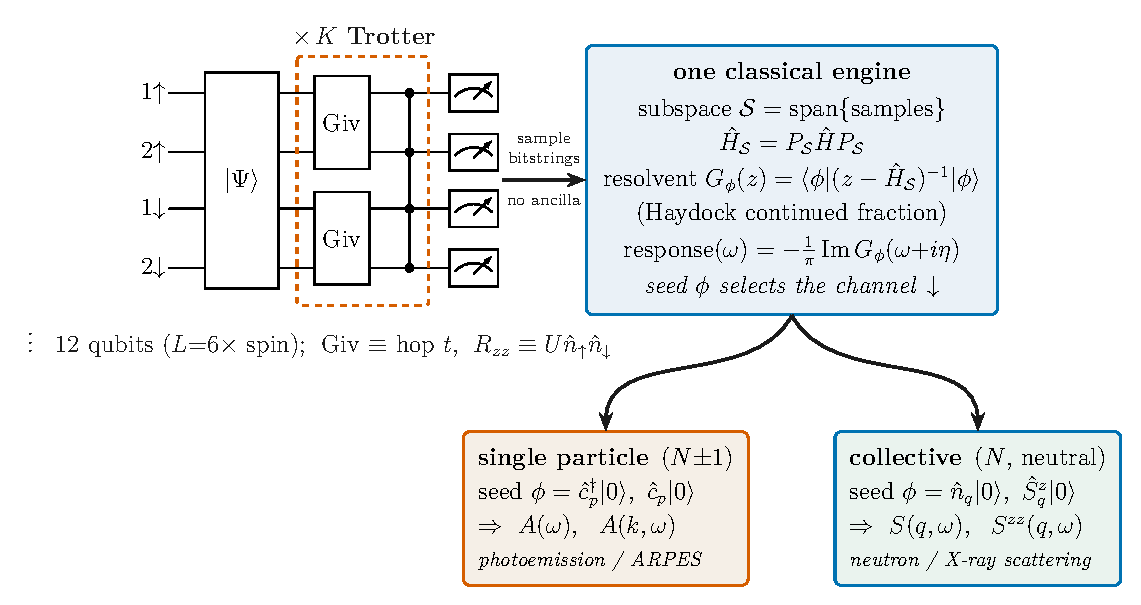
\includegraphics[width=\linewidth]{figs/fig_circuit.pdf}
\caption{\textbf{One sampling primitive, four dynamical responses.} A shallow, ancilla-free
circuit---state preparation and a Trotter layer repeated $K$ times (Givens rotations for the hopping
$t$, native $R_{zz}$ for the on-site $U\hat n_\uparrow\hat n_\downarrow$)---is measured in the
computational basis; no Hadamard test or controlled unitary is run on the device. The sampled
bitstrings define a sector-specific subspace $\mathcal S$ and feed a single classical engine---a Haydock
continued-fraction resolvent~\cite{haydock1972} $G_\phi(z)=\langle\phi|(z-\hat H_{\mathcal S})^{-1}|\phi\rangle$, whose
single-particle case ($\phi=\hat c^\dagger_p|0\rangle$) is the Green's function of
Eq.~\eqref{eq:green}. The seed $\phi$ then selects the channel: particle addition/removal seeds
$\hat c^{\dagger}_p|0\rangle,\hat c_p|0\rangle$ in the $(N{\pm}1)$ sectors give the single-particle
spectral functions $A(\omega)$ and $A(k,\omega)$ (photoemission/ARPES), while number-conserving density
and spin seeds $\hat n_q|0\rangle,\hat S^z_q|0\rangle$ in the $N$ sector give the dynamical structure
factors $S(q,\omega)$ and $S^{zz}(q,\omega)$ (neutron~\cite{squires2012} and resonant inelastic
X-ray~\cite{ament2011} scattering)---all from \emph{one} sampling
primitive, the seed selecting the sector and hence the subspace. The four channels are realized in Figs.~\ref{fig:method} ($A(\omega)$),
\ref{fig:lattice} ($A(k,\omega)$), \ref{fig:sqw} ($S(q,\omega)$), and \ref{fig:spin}
($S^{zz}(q,\omega)$).}\label{fig:circ}\end{figure*}
